\documentclass[xcolor=dvipsnames,table]{beamer}



\mode<presentation>{
  \usetheme{Warsaw}  
  
  \definecolor{INFblue}{HTML}{003087} % INFORMS blue
\definecolor{INFgreen}{HTML}{84BD00} % INFORMS green
\definecolor{INForange}{HTML}{E87722} % INFORMS orange
\definecolor{MYpurple}{HTML}{3c1361}
  
%  \usecolortheme{orchid} 
	\usecolortheme[named=MYpurple]{structure}
  \setbeamertemplate{navigation symbols}{}
  \setbeamertemplate{caption}[numbered]  
} 

\usepackage[english]{babel}
\usepackage[utf8x]{inputenc}
\usepackage{xcolor}
\usepackage{listings}
\lstset{
    language=[LaTeX]TeX,
    breaklines=true,
    basicstyle=\tt\scriptsize,
    keywordstyle=\color{blue},
    identifierstyle=\color{magenta},
}

\title[INFORMS 2021]{Using Mathematics to Study Partisan Gerrymandering in South Carolina}
%\subtitle{\textit{A Selection of Mathematical Applications}}
\author{\textbf{Anna Marie Vagnozzi}}
\institute{Clemson University \\ In collaboration with Matthew Saltzman}
\date{November 17, 2020}

\AtBeginSection[]{
  \begin{frame}<beamer>
    \frametitle{Outline}
    \tableofcontents[currentsection,currentsubsection]
  \end{frame}
}

\usepackage{dsfont}
\usepackage{amsmath}
\usepackage{amssymb,amsthm}
\usepackage{array}
\usepackage{stmaryrd}
\usepackage[all]{xy}
\usepackage{rotating}
\usepackage{pgfplots}
\usepgfplotslibrary{fillbetween}
\usetikzlibrary{patterns}
\pgfplotsset{width=6cm,compat=1.9}
\usepackage{multicol}
\usepackage[export]{adjustbox}
\usepackage{wrapfig}
\usepackage{hyperref}
\usepackage{mathdots}
\usepackage{movie15}

\newcommand{\msc}[1]{\mathds{#1}}
\newcommand{\Z}{\mathds{Z}}
\newcommand{\R}{\mathds{R}}
\newcommand{\N}{\mathds{N}}
\newcommand{\Q}{\mathds{Q}}
\newcommand{\C}{\mathds{C}}
\newcommand{\K}{\mathds{K}}
\newcommand{\cK}{\mathcal{K}}
\newcommand{\I}[1]{\mathfrak{#1}}
\newcommand{\kX}{\mathfrak{X}}
\newcommand{\m}{\mathfrak{m}}
\newcommand{\n}{\mathfrak{n}}
\newcommand{\p}{\mathfrak{p}}
\newcommand{\q}{\mathfrak{q}}
\newcommand{\bX}{\mathbf{X}}
\newcommand{\abs}[1]{\left|#1\right|}
\newcommand{\so}{\implies}
\newcommand{\set}[2]{\left\{ #1 \:|\: #2 \right\}}
\newcommand{\Span}[2]{\left\langle #1 \;|\; #2 \right\rangle}
\newcommand{\bso}{\Longleftarrow}
\newcommand{\ra}{\rightarrow}
\newcommand{\gen}[1]{\left\langle #1 \right\rangle}
\newcommand{\olin}[1]{\overline{#1}}
\newcommand{\ulin}[1]{\underline{#1}}
\newcommand{\Img}[1]{\text{Im}\left(#1\right)}
\newcommand{\Ker}[1]{\text{Ker}\left(#1\right)}
\newcommand{\coker}[1]{\operatorname{coker}\left(#1\right)}
\newcommand{\llra}{\longleftrightarrow}
\newcommand{\lra}{\longrightarrow}
\newcommand{\xra}[1]{\xrightarrow{#1}}
\newcommand{\wo}{\setminus}
\newcommand{\mcal}[1]{\mathcal{#1}}
\newcommand{\Aut}[1]{\text{Aut}\left(#1\right)}
\newcommand{\Inn}[1]{\text{Inn}\left(#1\right)}
\newcommand{\syl}[2]{\text{Syl}_{#1}(#2)}
\newcommand{\norm}[1]{\left\|#1\right\|}
\newcommand{\infnorm}[1]{\left\|#1\right\|_{\infty}}
\newcommand{\xn}{\{x_n\}}
\newcommand{\sig}{\sigma}
\newcommand{\id}{\text{id}}
\newcommand{\ep}{\epsilon}
\newcommand{\st}{\text{ s.t. }}
\newcommand{\ran}[1]{\text{Ran}(#1)}
\newcommand{\nCr}[2]{\binom{#1}{#2}}
\newcommand{\pf}{\subparagraph{Proof:}}
\newcommand{\Homur}{\operatorname{Hom}_{U^{-1}R}}
\newcommand{\Homr}[1][R]{\operatorname{Hom}_{#1}}
\newcommand{\Extr}[2][R]{\operatorname{Ext}_{#1}^{#2}}
\newcommand{\Tor}[2][R]{\operatorname{Tor}^{#1}_{#2}}
\newcommand{\soc}{\operatorname{Soc}}
\newcommand{\edim}{\text{edim}}
\newcommand{\dep}[2]{\operatorname{depth}_R(#1;#2)}
\newcommand{\ce}{\:\colon\!\!\!\!=\:}
\newcommand{\del}{\nabla}
\newcommand{\spec}{\operatorname{Spec}}
\newcommand{\rad}{\operatorname{rad}}
\newcommand{\mrad}{\operatorname{m-rad}}
\newcommand{\ann}[1][R]{\operatorname{Ann}_{#1}}
\newcommand{\supp}[1][R]{\operatorname{Supp}_{#1}}
\newcommand{\ass}[1][R]{\operatorname{Ass}_{#1}}
\newcommand{\zd}[1][R]{\operatorname{ZD}_{#1}}
\newcommand{\nzd}[1][R]{\operatorname{NZD}_{#1}}
\newcommand{\Min}[1][]{\operatorname{Min}_{#1}}
\newcommand{\pdr}[1][R]{\operatorname{pd}_{#1}}
\newcommand{\cone}{\operatorname{Cone}}
\newcommand{\koz}[1][\bullet]{\operatorname{K}_{#1}}
\newcommand{\So}{\mathcal{S}_0}
\newcommand{\tens}[1][R]{\underset{#1}{\otimes}}
\newcommand{\type}{\operatorname{type}}

\newcommand {\framedgraphic}[2] {
    \begin{frame}{#1}
        \begin{center}
%            \includegraphics[width=\textwidth,height=0.8\textheight,keepaspectratio]{#2}
        \end{center}
    \end{frame}
}

\newcolumntype{L}{>{$}l<{$}}
\theoremstyle{plain}
\newtheorem{thm}{Theorem}
\newtheorem{lem}[thm]{Lemma}
\newtheorem{prop}[thm]{Proposition}
%\newtheorem{fact}[thm]{Fact}
\newtheorem{cor}[thm]{Corollary}
\newtheorem{facdef}[thm]{Fact/Definition}
\newtheorem{law}{Law}
\theoremstyle{definition}
\newtheorem{ex}[thm]{Example}
\newtheorem{defn}[thm]{Definition}
%\newtheorem{note}[thm]{Note}
\newtheorem{notn}[thm]{Notation}
\newtheorem{disc}[thm]{Discussion}
\newtheorem{rmk}[thm]{Remark}
\newtheorem{rec}[thm]{Recall}
\newtheorem{con}[thm]{Construction}
\newtheorem{prob}[thm]{Open Problem}

%\bibliographystyle{amsplain}

%%%%%%%%%%%%%%%%%%%%%%%%%%%%%%%%%%%%%%%%%%%%%%%%%%%%%%%%%%%%%%%%%%%%%%%

\begin{document}

%---------------------------------------------------------------------
%\begin{frame}
%  \titlepage
%\end{frame}

%---------------------------------------------------------------------

%\section*{Background}

%---------------------------------------------------------------------

%\textcolor{MYpurple}{\scriptsize \textit{League of Women Voters of Pennsylvania, et al.\ v.\ Commonwealth of Pennsylvania, et al.}, No.\ 159 MM 2017 (2018)}

%---------------------------------------------------------------------

\begin{frame}{Congressional Maps}

\begin{minipage}{0.5\textwidth}
\hspace{-8mm}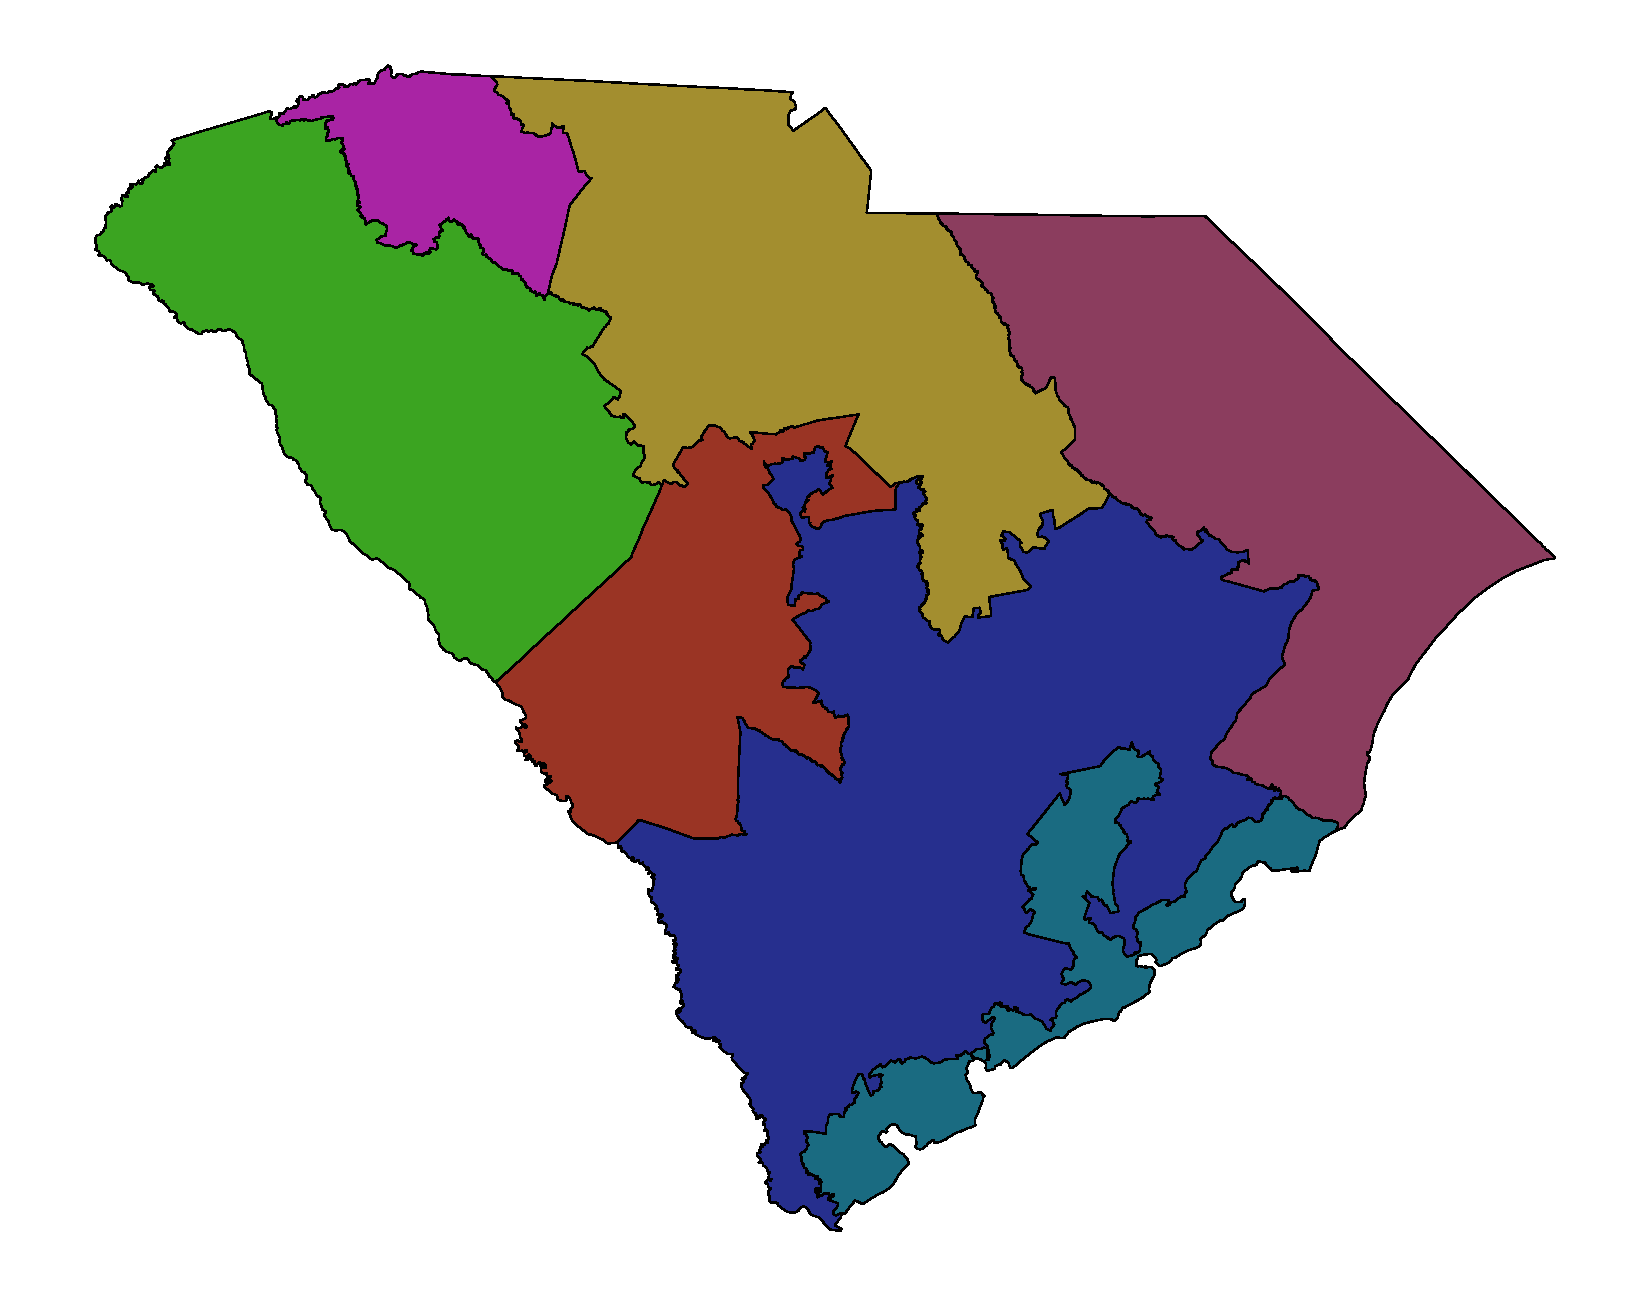
\includegraphics[scale=.25]{Congress2011.pdf}
2011 Congressional Districts
\end{minipage}%
\begin{minipage}{0.5\textwidth}
\hspace{-5mm}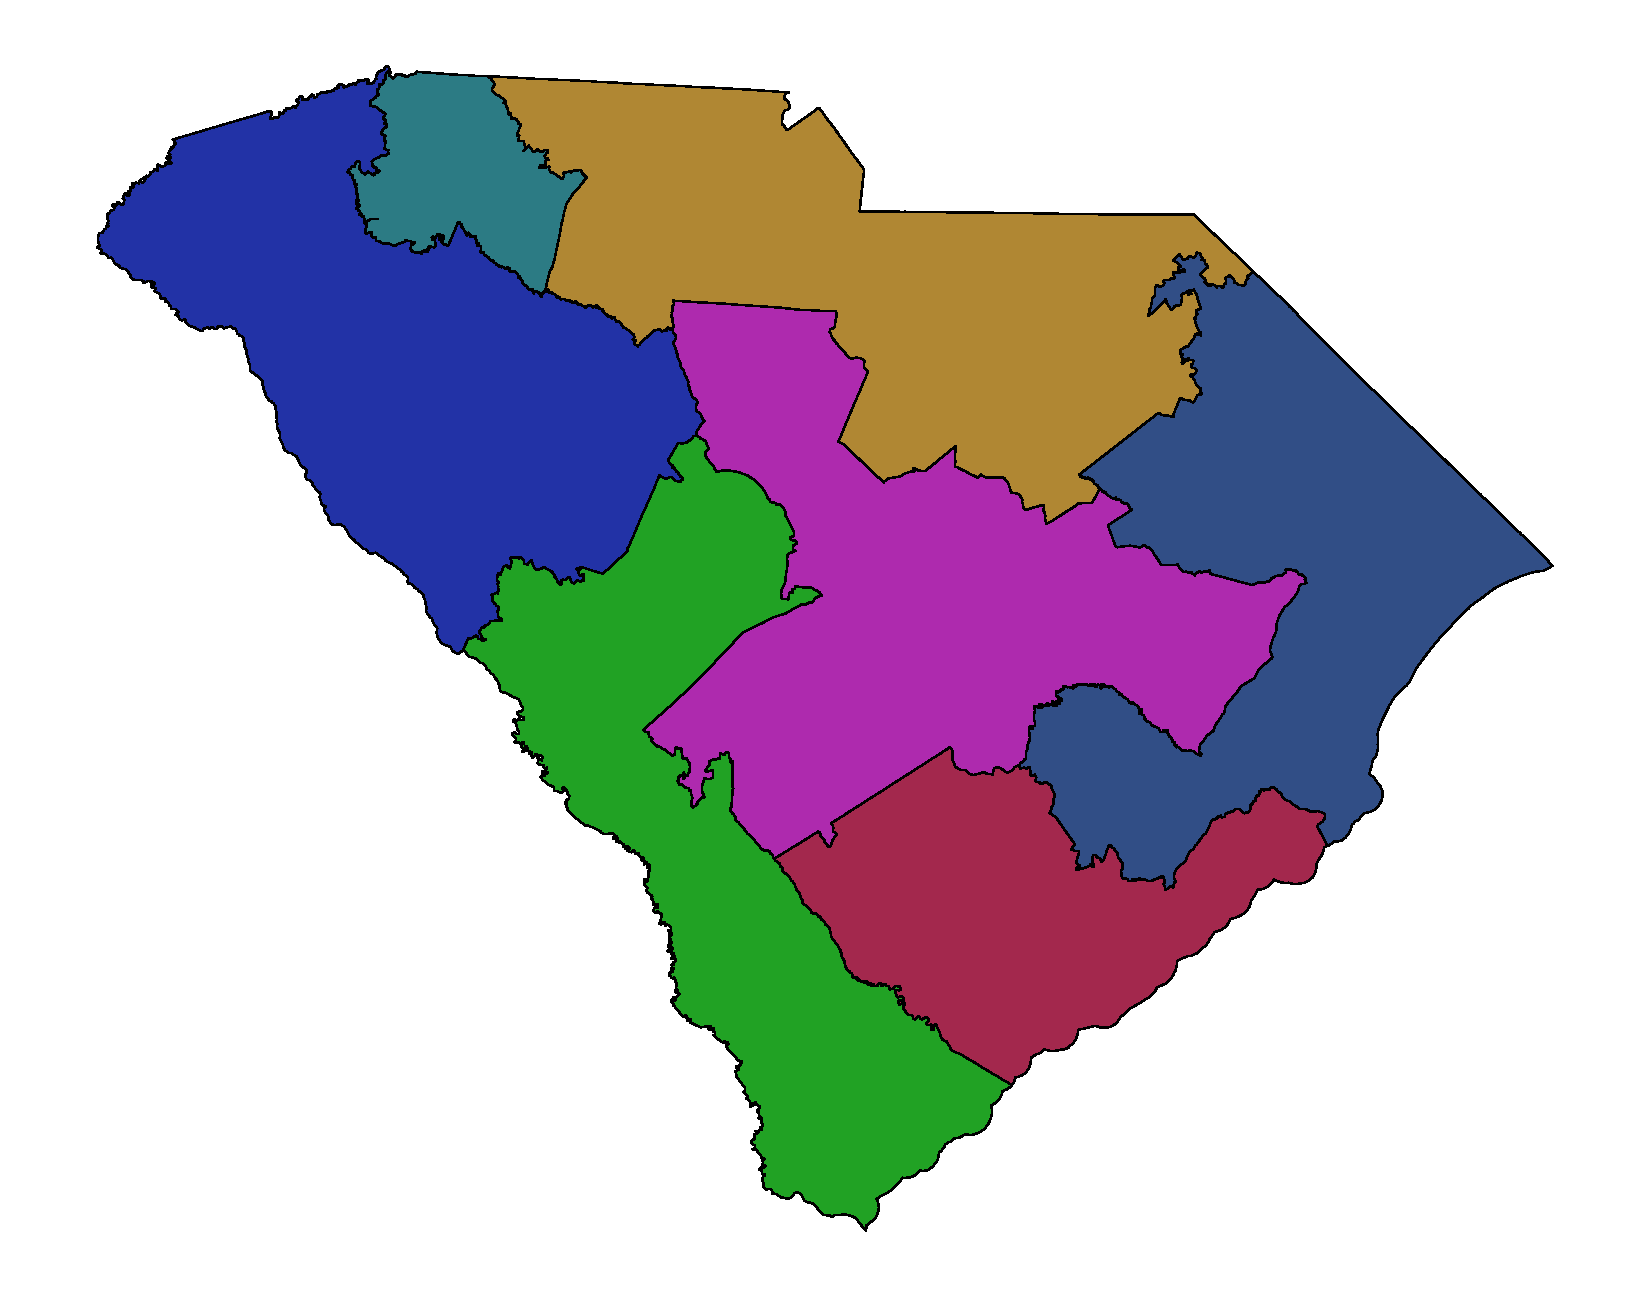
\includegraphics[scale=0.25]{Congress2021.pdf}

%\vspace{-4mm}

\hspace{10mm}Proposed LWV Districts
\end{minipage}
\end{frame}

\begin{frame}{State Senate Maps}
\begin{minipage}{0.5\textwidth}
\hspace{-8mm}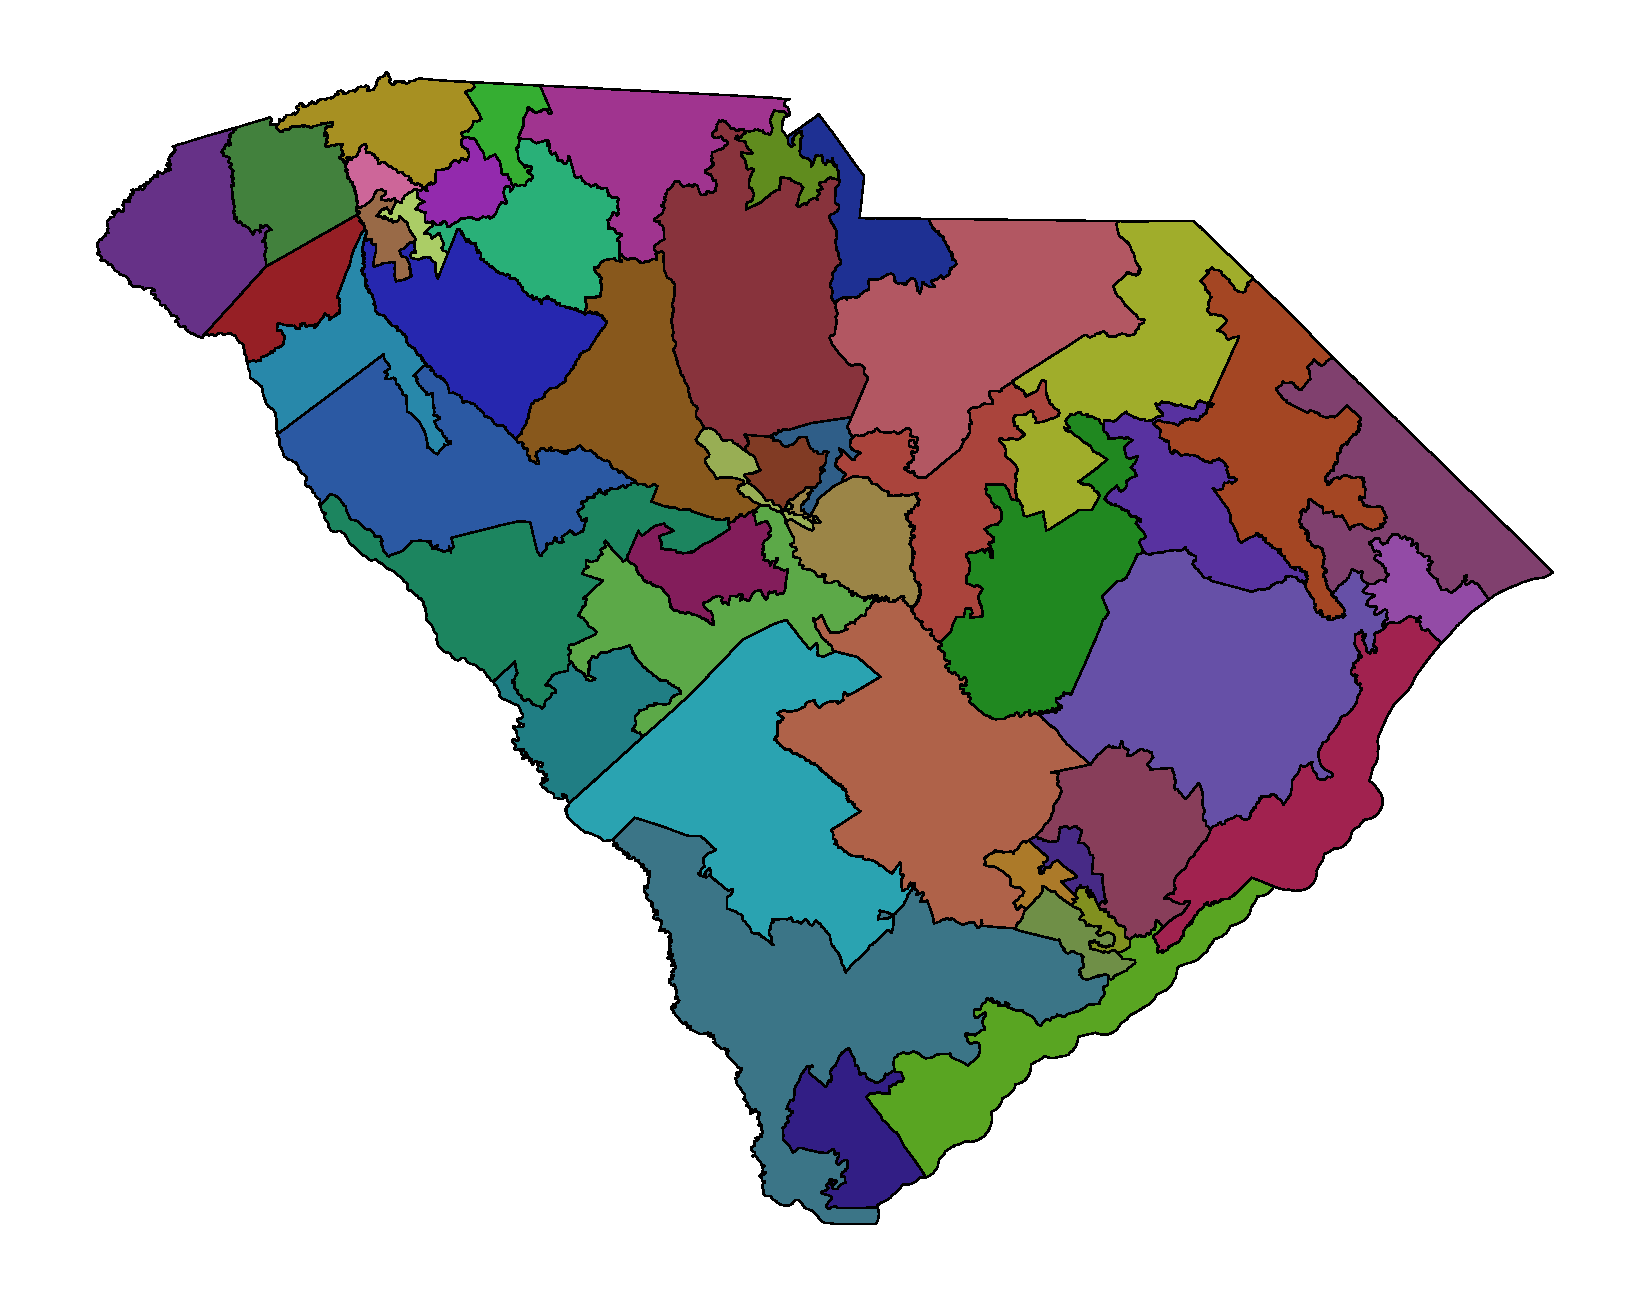
\includegraphics[scale=0.26]{Senate2011.pdf}
\hspace{25mm}2011 Senate Districts
\end{minipage}%
\begin{minipage}{0.5\textwidth}
\hspace{-5mm}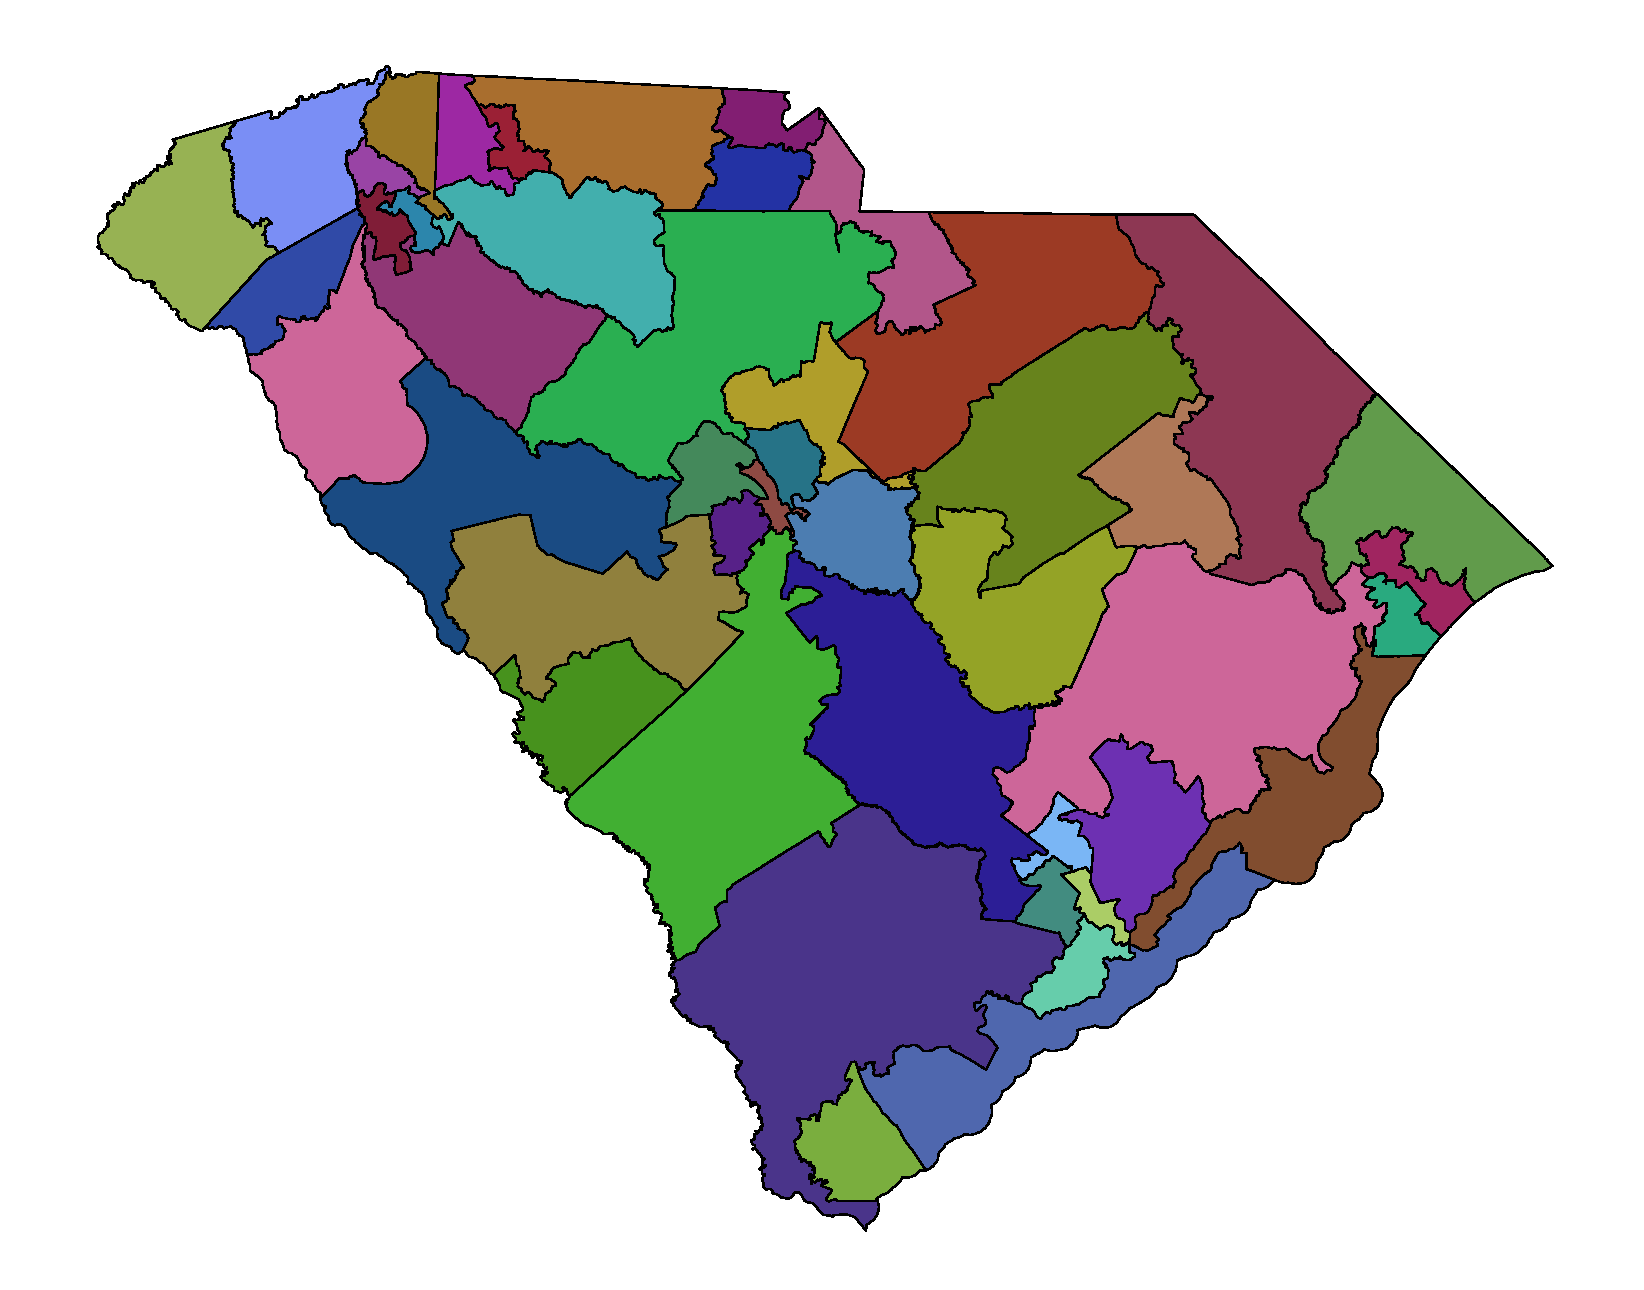
\includegraphics[scale=0.26]{Senate2021.pdf}

%\vspace{3mm}

\hspace{10mm} Proposed LWV Districts
\end{minipage}
\end{frame}

\begin{frame}{State House Maps}
\begin{minipage}{0.5\textwidth}
\hspace{-9mm}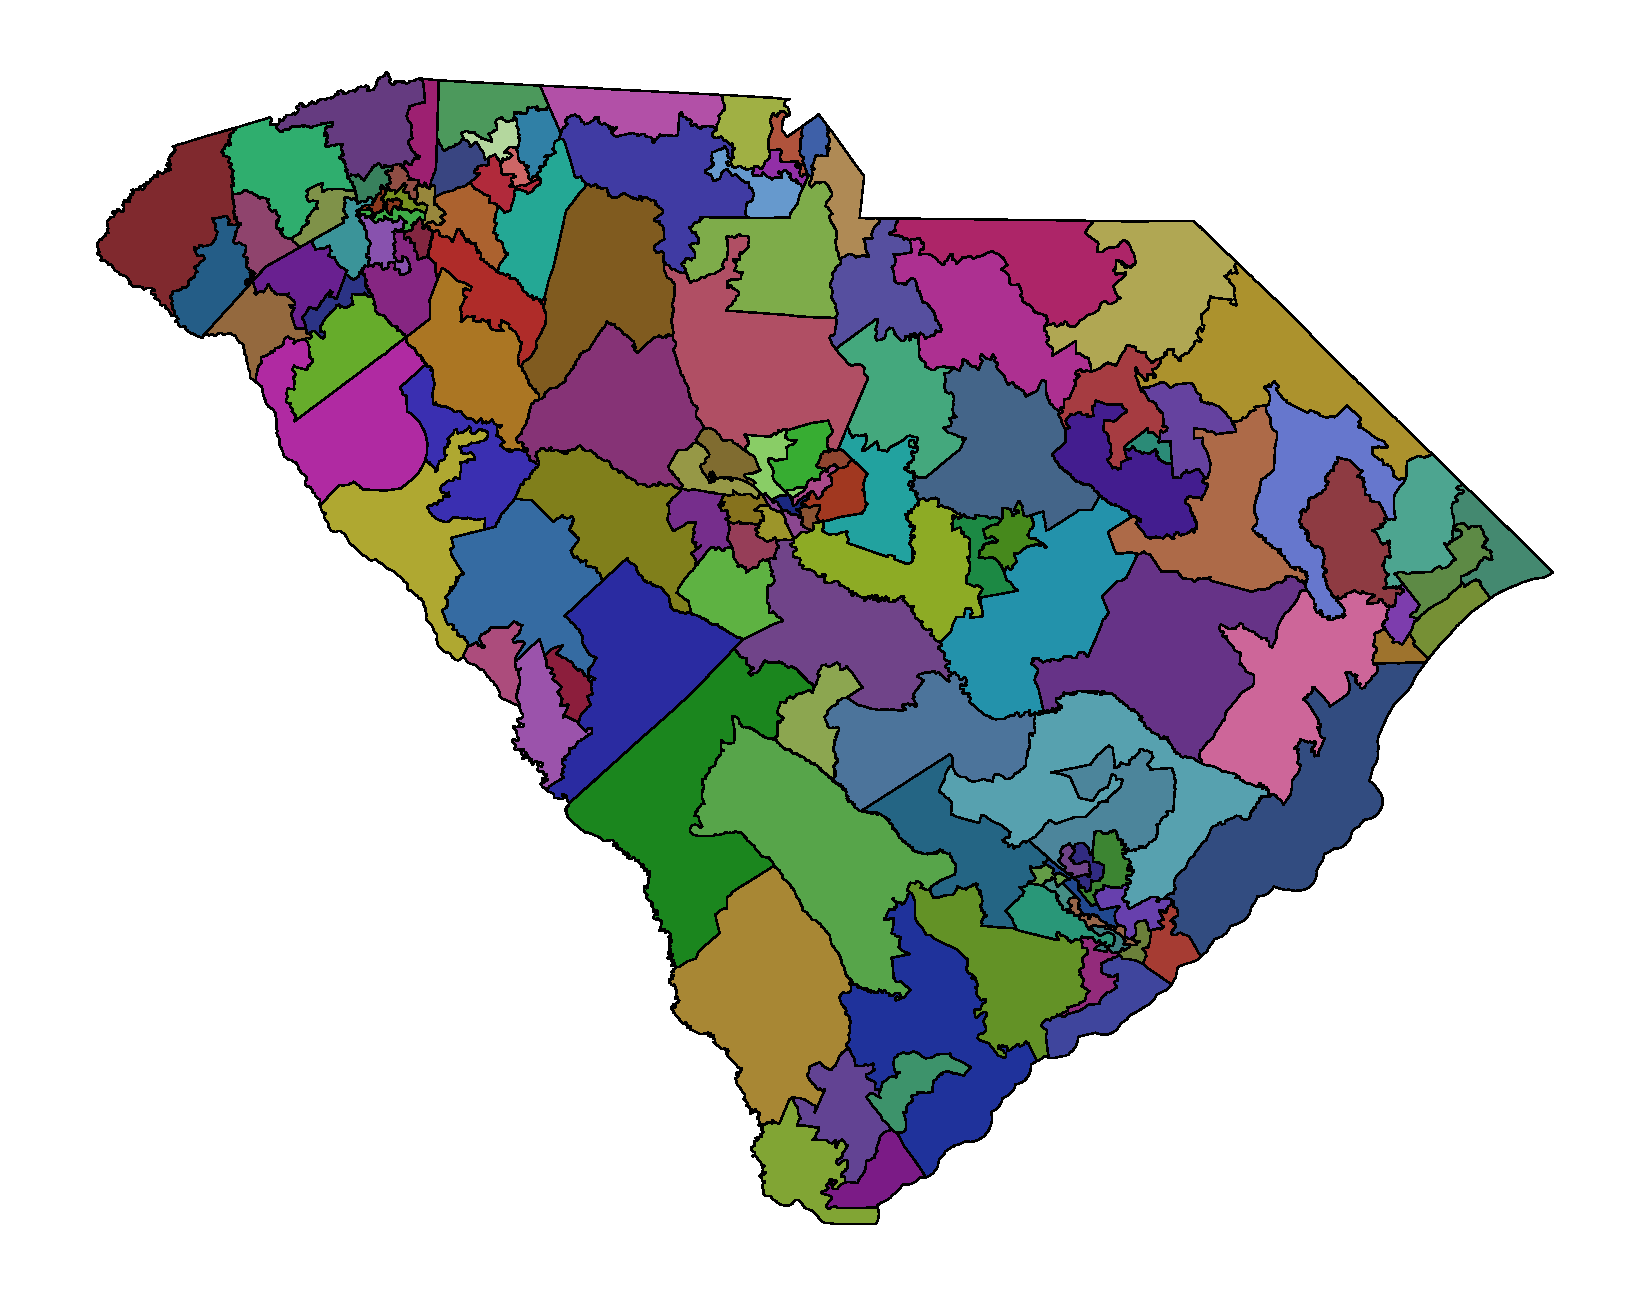
\includegraphics[scale=0.26]{House2011.pdf}

\hspace{5mm} 2011 House Districts
\end{minipage}%
\begin{minipage}{0.5\textwidth}
\hspace{-8mm} 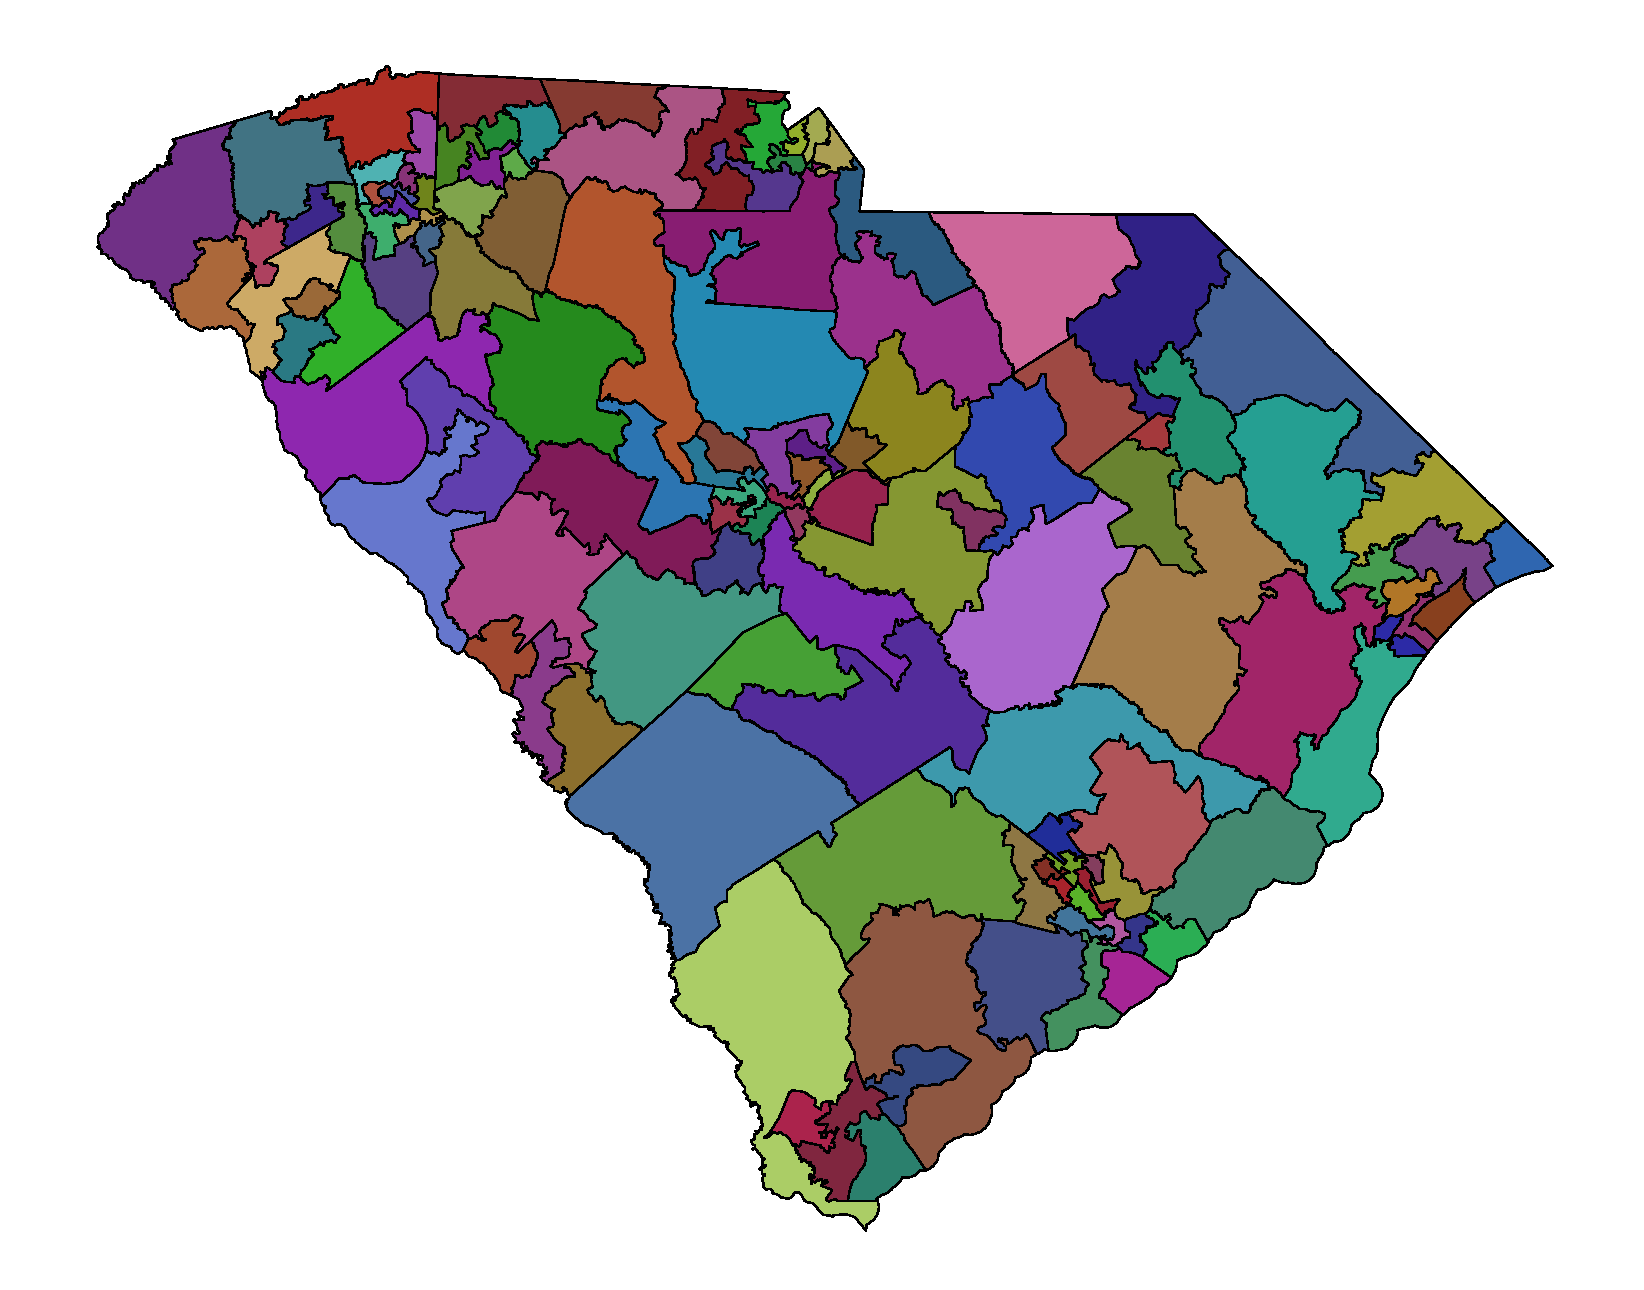
\includegraphics[scale=0.26]{House2021.pdf}

%\vspace{-1mm}

\hspace{8mm} Proposed LWV Districts
\end{minipage}
\end{frame}


\begin{frame}{Bias Analyses for South Carolina Maps}
		\mbox{Two reliable measures of partisan bias are used to assess each map.}
		
		\begin{defn}
		\small Let $V^O$ be the observed statewide average district vote and let $M$ be the median district vote share. The \textbf{median-mean} metric is defined as $$\textsc{MM}=M-V^O.$$
		$\textsc{MM}<0$ indicates an advantage for Republicans.
		\end{defn}
		
		\begin{defn}
	\small	\textbf{Geometric partisan bias} is defined as 
		$$B_G=\int_0^1\Big|\widehat{S}(v)-\widehat{S}^{-1}(v)\Big|dv,$$
		where $\widehat{S}(V)$ is the estimated seats-votes curve using a variable partisan swing assumption and $\widehat{S}^{-1}(V)$ is this curve inverted around the $(0.5,0.5)$ midpoint.
		\end{defn}
\end{frame}

%------------------------------

\begin{frame}{Bias Analyses for South Carolina Maps}

Both \textbf{median-mean} and \textbf{geometric bias} satisfy the partisan symmetry standard.

\vspace{3mm}

Median-mean indicates the \textbf{direction} of the bias, while geometric bias characterizes \textbf{overall} bias in either party direction.

\vspace{3mm}

Though not a measure of partisan symmetry, average district \textbf{efficiency gap} was also considered to characterize wasted votes. 

\vspace{2mm}

\begin{defn}
\small For two Parties $D$ and $R$, the \textbf{efficiency gap} is computed as
$$\textsc{EG}=\frac{\left(\ell_D+w_D\right)-\left(\ell_R+w_R\right)}{N},$$

where $\ell$ is the number of votes cast for a losing candidate, $w$ is the number of votes cast for a winning candidate above the threshold of 50\% plus one vote, and $N$ is the total number of votes cast. $EG>0$ indicates that Party $D$ wasted more votes than Party $R$.
\end{defn}

\end{frame}

%------------------------------

\begin{frame}{Bias Analyses for South Carolina Maps}
\begin{itemize}
	\item Bias analyses are currently being conducted for  Congressional, SC Senate, and SC House districting plans.
	\item Precinct-level geography and voting data corresponding to the 2020 General Election were utilized for the analysis.
	\item The U.S.\ Senate race (Graham vs.\ Harrison) was utilized as a proxy for statewide voter preferences.
	\item Comparative analyses were run for the 2011 redistricting plans from last year and the proposed 2021 plans provided by the SC League of Women Voters.
\end{itemize}
\end{frame}

%------------------------------

\begin{frame}{Congressional Maps (7 Districts)}
	
\renewcommand{\arraystretch}{1.5}
	
\begin{center}
\begin{table}[]
\begin{tabular}{|c|c|c|}
\hline
\textbf{}               & \textbf{\begin{tabular}[c]{@{}c@{}}Original 2011 Map\end{tabular}} & \textbf{\begin{tabular}[c]{@{}c@{}}Proposed 2021 Map\end{tabular}} \\ \hline
\textbf{Median-Mean}    & $-0.0238$                                                               & \cellcolor[HTML]{FFCCC9}$-0.0343$                                      \\ \hline
\textbf{Geometric Bias} & $0.0231$                                                                & \cellcolor[HTML]{FFCCC9}$0.0352$                                       \\ \hline
\textbf{Efficiency Gap} & 0.2624                                                                & \cellcolor[HTML]{C6ECC6}0.1104                                       \\ \hline
\end{tabular}
\end{table}
\end{center}
	
	\vspace{3mm}
	
Compared to the existing districting plan from 2011, the proposed Congressional map by LWV fares better in terms of efficiency gap, but worse in terms of both partisan bias measures.
	
\end{frame}

\begin{frame}{SC Senate Map (46 districts)}

\begin{center}

\renewcommand{\arraystretch}{1.5}

\begin{table}[]
\begin{tabular}{|c|c|c|}
\hline
\textbf{}               & \textbf{\begin{tabular}[c]{@{}c@{}}Original 2011 Map\end{tabular}} & \textbf{\begin{tabular}[c]{@{}c@{}}Proposed 2021 Map\end{tabular}} \\ \hline
\textbf{Median-Mean}    & $-0.0328$                                                               & \cellcolor[HTML]{FFCCC9}$-0.0355$                                      \\ \hline
\textbf{Geometric Bias} & $0.0301$                                                                & \cellcolor[HTML]{C6ECC6}$0.02671$                                       \\ \hline
\textbf{Efficiency Gap} & $0.0685$                                                                & \cellcolor[HTML]{FFCCC9}$0.0815$                                       \\ \hline
\end{tabular}
\end{table}
\end{center}

\vspace{3mm}

Compared to the existing districting plan from 2011, the proposed State Senate map by LWV fares better in terms of geometric bias. It is worse in terms of efficiency gap, but only slightly worse in terms of median-mean.
\end{frame}

\begin{frame}{SC House Map (124 districts)}


\begin{center}
\renewcommand{\arraystretch}{1.5}

\begin{table}[]
\begin{tabular}{|c|c|c|}
\hline
\textbf{}               & \textbf{\begin{tabular}[c]{@{}c@{}}Original 2011 Map\end{tabular}} & \textbf{\begin{tabular}[c]{@{}c@{}}Proposed 2021 Map\end{tabular}} \\ \hline
\textbf{Median-Mean}    & $-0.0445$                                                               & \cellcolor[HTML]{C6ECC6}$-0.0280$                                      \\ \hline
\textbf{Geometric Bias} & $0.0411$                                                                & \cellcolor[HTML]{C6ECC6}$0.0344$                                       \\ \hline
\textbf{Efficiency Gap} & $0.0976$                                                                & \cellcolor[HTML]{C6ECC6}$0.0837$                                       \\ \hline
\end{tabular}
\end{table}
\end{center}

\vspace{3mm}

Compared to the existing districting plan from 2011, the proposed State House map by LWV fares better with respect to all three measures.
\end{frame}

%------------------------------

\begin{frame}{References}

	\textcolor{MYpurple}{\scriptsize \textbf{Markov Chain Analysis:} Maria Chikina, Alan Frieze, and Wesley Pegden, \textit{Assessing significance in a Markov chain without mixing,} Proceedings of the National Academy of Sciences 114 (2017), no.\ 11, 2860--2864.}

\vspace{2mm}
	\textcolor{MYpurple}{\scriptsize \textbf{Partisan Symmetry:} Jonathan N.\ Katz, Gary King, and Elizabeth Rosenblatt, \textit{Theoretical foundations and empirical evaluations of partisan fairness in district-based democracies,} American Political Science Review (2019), 1--15.}

\vspace{2mm}	
	\textcolor{MYpurple}{\scriptsize \textbf{Geometric Bias:} John F.\ Nagle, \textit{Measures of partisan bias for legislating fair elections}, Election Law Journal 14(2015), no.\ 4, 346--360.}
	
	\vspace{2mm}
	
	\textcolor{MYpurple}{\scriptsize \textbf{Thesis (demonstrating equivalent performance of Geometric Bias under outlier analysis):} Anna Marie Vagnozzi, \textit{Detecting partisan gerrymandering through mathematical analysis: A case study of South Carolina,} TigerPrints: Theses and Dissertations (2020).}

\end{frame}

%---------------------------------------------------------------------

\end{document}
